\capitulo{Técnicas y herraminetas}
\label{cha:Técnicas y herraminetas}

\section{Herramientas de desarrollo}

Este capítulo detalla las distintas herramientas, librerías y frameworks que se
han utilizado durante el desarrollo del proyecto.

\subsection{Windows Subsystem for Linux}

Windows Subsystem for Linux (WSL) es una utilidad creada principalmente por
Microsoft y Canonical (Mantenedores de Ubuntu) que permite utilizar un sistema
operativo Linux desde Windows sin grandes pérdidas de rendimiento. Existen
varias opciones de distribución que se pueden utilizar (Kali Linux, OpenSUSE,
etc.), pero la mas utilizada y mejor mantenida para WSL es Ubuntu, por lo que es
la que se ha utilizado.

La mayor parte del desarrollo ha sido realizada desde WSL, donde se ha instalado
tanto \LaTeX{} como Python 3.9 y algunas dependencias, proceso mucho más simple
de realizar en Linux que en Windows.

\subsection{Python}


\subsection{Visual Studio Code}

Visual Studio Code (VS Code) es un popular editor de texto altamente extensible
orientado al desarrollo creado por Microsoft. Gracias a su gran extensibilidad
es posible utilizarlo cómodamente en casi cualquier escenario. Mediante una de
estas extensiones (denominada literalmente WSL) se puede conectar con WSL y
utilizar los programas que tiene instalados como si hubiese sido ejecutado
diréctamente desde un sistema operativo Linux.

En este caso se ha utilizado VS Code para:

\begin{itemize}
      \item Crear tanto esta memoria como los anexos mediante la extensión
            \href{https://github.com/James-Yu/LaTeX-Workshop}{\LaTeX{} Workshop}
            que integra distintos compiladores de \LaTeX{} (pdfTeX, XeTeX, LuaTeX,
            etc.) dentro del programa y añade otras funcionalidades que hacen la
            edición de código \LaTeX{} mucho más conveniente.
      \item Crear la aplicación web, que utiliza el framework de JavaScript
            SvelteKit, mediante multitud de extensiones para integrar la multitud
            de librerías utilizadas (Svelte, TypeScript, Prettier, etc.).
      \item Editar archivos de configuración utilizados para la creación de los
            contenedores de Docker que componen la totalidad de la aplicación web
            (web, API y proxy inverso).
\end{itemize}


\subsection{PyCharm}

PyCharm es un Entorno de Desarrollo Integrado (IDE, por sus siglas en inglés)
creado y mantenido por JetBrains, una compañía que se dedica a crear software y
cuyos productos más representativos son multitud de IDEs para diferentes
lenguajes de programación (IntelliJ (Java), CLion (C y C++), GoLand (Go), etc.).

El objetivo de PyCharm es facilitar el desarrollo de aplicaciones que utilizad
Python y da soporte amplio tanto para los habituales ficheros \texttt{.py} como
para \texttt{.ipynb} (Notebooks de Jupyter), que han sido utilizados
extensamente en el proyecto.

Además, PyCharm por defecto permite la integración con entornos WSL de forma muy
fácil, simplemente se le debe indicar la localización del ejecutable de Python
en el sistema de archivos de la distribución de WSL.

En este proyecto PyCharm se ha utilizado para:

\begin{enumerate}
      \item Desarrollar la librería PADDEL, que contiene el código de Python común
            a los Notebooks de Jupyter utilizados durante la fase de investigación
            y a la aplicación web.
      \item Desarrollar la API que utiliza la aplicación web.
\end{enumerate}


\subsection{Git}

Actualmente Git es el sistema de control de versiones más extendido en proyectos
de código abierto \cite{OpenHubVCS}, en este proyecto se ha usado para gestionar
y guardar de forma segura los cambios que se han ido realizado con el tiempo en
la plataforma GitHub.

Aunque existen varias herramientas con interfaces gráficas que envuelven el
funcionamiento de Git (GitKraken, GitHub Desktop, etc.) para este proyecto se ha
utilizado directamente el comando \texttt{git} desde una terminal de WSL.


\subsection{OpenCV}

OpenCV es una librería de visión artificial que contine varias utilidades para
interactuar con archivos de vídeo e imágenes de forma similar a como se
trabajaría en un programa como MATLAB. OpenCV está escrito en C y C++ pero tiene
\textit{bindings} que permiten interactuar con sus APIs desde Python.

En este proyecto se usa para leer y decodificar los archivos de vídeo
utilizados.


\subsection{MediaPipe}

MediaPipe es una librería de aprendizaje automático mantenida por Google que da
acceso a varios modelos preentrenados que se centran en la detección de
características corporales a partir de flujos de imágenes, en este caso se
utilizó MediaPipe Hands, cuyo objetivo es extraer varios puntos que definen un
esqueleto ligeramente simplificado de la mano humana.

\begin{figure}[h]
      \centering
      \subfloat{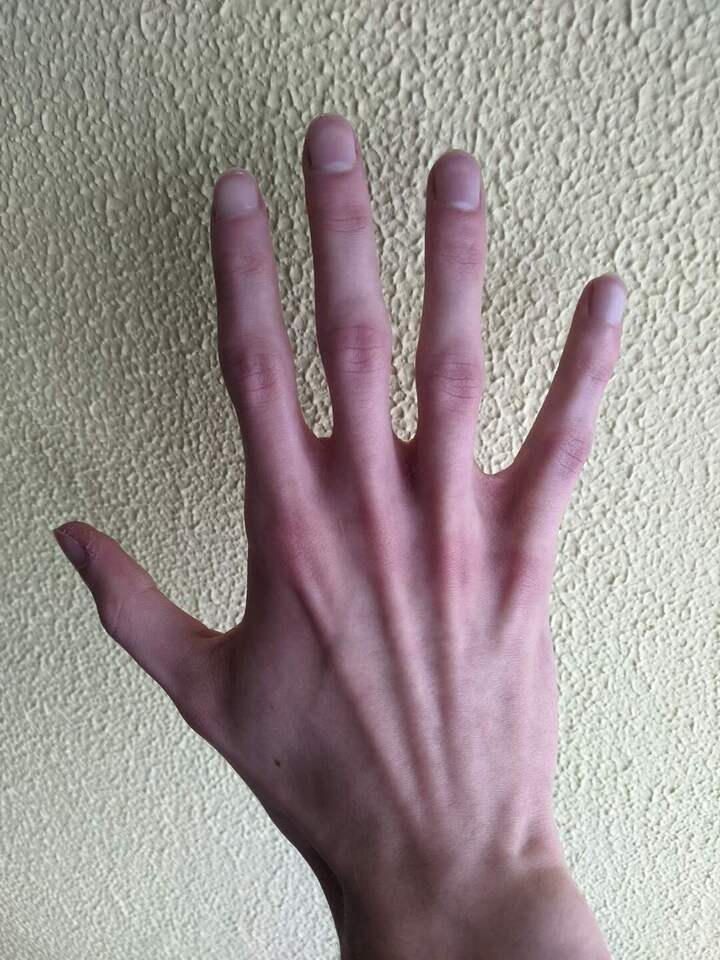
\includegraphics[width=0.33\textwidth]{herramientas_desarrollo/mano.jpg}}
      \subfloat{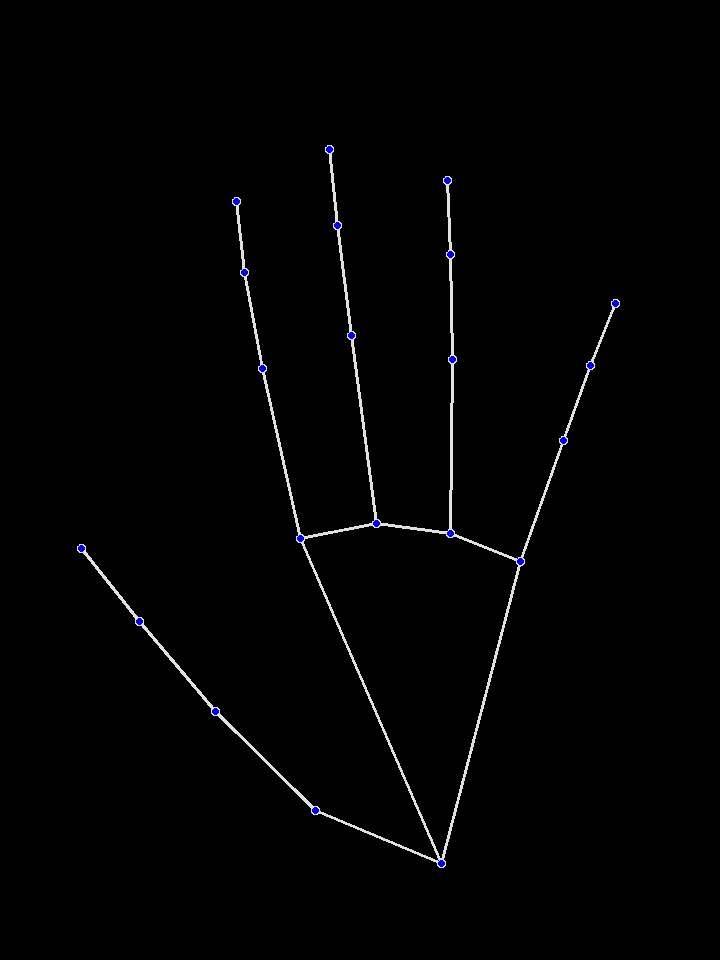
\includegraphics[width=0.33\textwidth]{herramientas_desarrollo/pose.jpg}}
      \subfloat{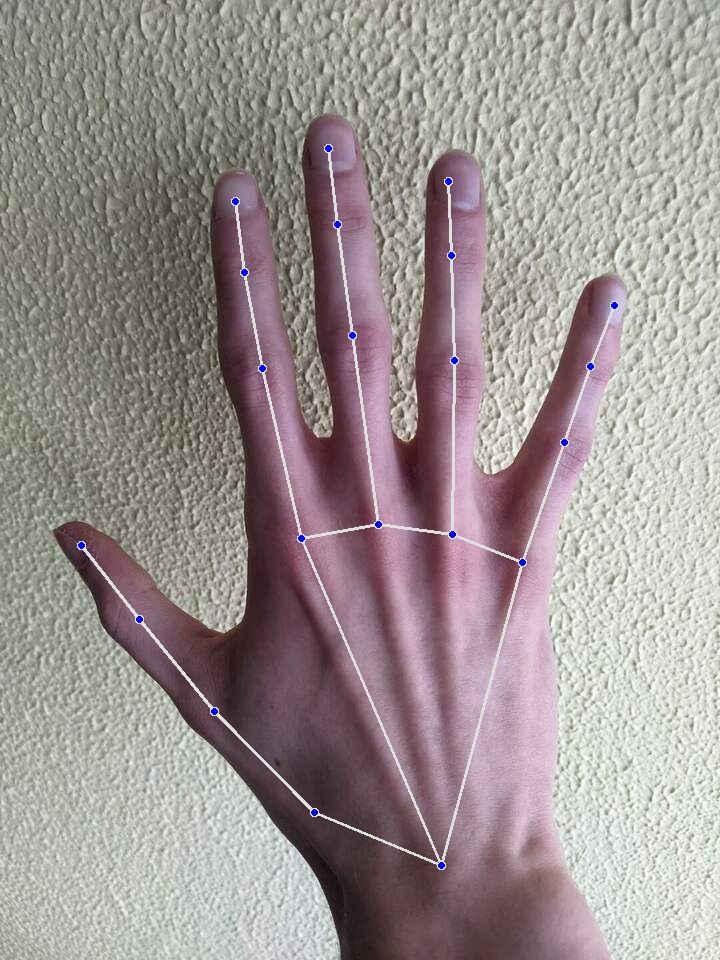
\includegraphics[width=0.33\textwidth]{herramientas_desarrollo/mano_pose.jpg}}
      \caption{MediaPipe Hands}
\end{figure}


\subsection{FastAPI}

FastAPI es un \textit{framework} de Python utilizado para crear APIs de tipo
REST que se caracteriza por permitir al programador centrar sus esfuerzos en el
código relacionado con la lógica de negocio al realizar la mayoría de acciones
comunes entre diferentes APIs por defecto (como la creación de documentación,
validación de tipos, serialización y deserialización de peticiones, etc.).

En este proyecto se ha creado una API REST para permitir la interacción con el
código de Python utilizado para crear, entrenar y utilizar los modelos desde
cualquier dispositivo y lenguaje de programación (siempre y cuando permita
realizar peticiones HTTP). Con esto se consigue que en el futuro se puedan crear
nuevas formas para interactuar con los modelos sin necesidad de alterar el
código ya existente, por ejemplo, se podría crear una aplicación móvil para
facilitar la toma y subida de vídeos. Además estas nuevas aplicaciones podrían
estar creadas por personas ajenas al proyecto que necesiten una implementación
diferente para su caso de uso específico.


\subsection{NextJS}


\subsection{Caddy}

En las fases iniciales de desarrollo se decidió que la API debería estar alojada
en la ruta \texttt{/api}, mientras el resto de rutas debería llevar a la web
(SvelteKit). Esto significa que van a existir dos servicios funcionando de forma
paralela (Web y API), y que dependiendo de la ruta a la que se realize una
petición, ésta debería ser redirigida a un servicio u otro.

Esta situación es uno de los casos de uso idóneos para un proxy inverso, que es
un servicio que recibe peticiones HTTP, las altera si es necesario, y las
redirige al servicio de destino (el cual se determina mediante ciertas reglas de
redirección).

En un principio se optó por utilizar Nginx para implementar este proxy inverso
con muy buenos resultados gracias a su fácil configuración, rendimiento y
simplicidad. Pero surgieron problemas al añadir soporte para utilizar
certificados SSL y realizar peticiones seguras mediante HTTPS, ya que era
deseable una solución que gestionase de forma automática la petición y
renovación de estos certificados y Nginx, debido a su simplicidad no dispone de
esta funcionalidad.

Se probaron dos alternativas que solucionaban este problema, Traefik y Caddy,
ambas escritas en GoLang. Traefik dispone de una gran cantidad de
funcionalidades incluyendo gestión de certificados SSL, entre muchas otras, como
un panel de control desde el que visualizar estadísticas sobre el nivel de uso
del servicio.

La otra alternativa, Caddy, es mucho más simple, pero realiza la gestión de
certificados de forma automática por defecto, e incluso permite el uso de
certificados \textit{self-signed} (firmados por uno mismo, en lugar de por una
entidad certificadora). Esto es de gran utilidad durante el desarrollo para
asegurar que el funcionamiento de la aplicación va a seguir siendo el mismo en
el entorno final de producción (ya que hay ligeras diferencias dependiendo de si
un navegador utiliza HTTP o HTTPS).

Es por todo lo anterior que, al final, se decidió usar Caddy.


\subsection{Docker}

Docker es una herramienta que permita la creación y gestión de contenedores de
sistemas operativos aislados del sistema anfitrión y entre sí con un
\textit{overhead} my pequeño con respecto a una ejecución nativa.

En este caso se ha utilizado Docker para facilitar el despliegue de la
aplicación web, con tres contenedores (API, web y proxy inverso), en cualquier
máquina que disponga de Docker. La única configuración que se debe realizar para
desplegar la aplicación es la creación de un archivo de variables de entorno
(\texttt{.env}) en el que se definen valores específicos al entorno (nombre de
dominio, puertos en los que escuchar las peticiones).

Docker permite la creación de redes locales de contenedores, en este caso se
utiliza una de estas redes para permitir la conexión entre los tres contenedores
como si fuesen máquinas distintas conectadas a una misma red local donde la
única máquina (contenedor) con conexión al exterior es la que está ejecutando el
servicio del proxy inverso, por el que tienen que pasar todas las peticiones
antes de llegar al servicio de API o al de web.


\subsection{Formateado del código}

Se han utilizado las siguientes herramientas para realizar el formateado del
código escrito en Python de forma automática:

\begin{itemize}
      \item \textbf{Autoflake}: herramienta utilizada para la eliminación de
            sentencias \texttt{import} y variables innecesarias.
      \item \textbf{Isort}: herramienta para la reordenación de sentencias
            \texttt{import}.
      \item \textbf{Black}: formateador de código caracterizado por un enfoque en
            convenciones, por esto permite una configuración muy limitada por
            parte del usuario.
\end{itemize}


\subsection{Make}

A través del proyecto hay comandos de cierta complejidad que se repiten con
bastante frecuencia (\textit{e.g.} formatear el código, lanzar contenedores, limpiar
contenedores, etc.), para facilitar el uso de estos comandos se ha utilizado la
utilidad GNU Make, que viene por defecto en la mayoría de sistemas operativos de
tipo Linux y se puede instalar tanto en Windows como en MacOS.

El funcionamiento de Make consiste en la creación de un archivo denominado
\texttt{Makefile} que contiene diferentes comandos y secuencias de comandos con
las dependencias que existen entre los mismos.

Por ejemplo:

\begin{verbatim}
format:
    autoflake src
    isort src
    black src
\end{verbatim}

Un fichero \texttt{Makefile} con el contenido anterior permite ejecutar el
comando \texttt{make format} (siempre desde el mismo directorio en el que se
encuentra \texttt{Makefile}) para ejecutar la secuencia de comandos denominada
\texttt{format}, que, en este caso ejecutará varios comandos para realizar un
formato del código.
